\documentclass[tikz]{standalone}
\begin{document}

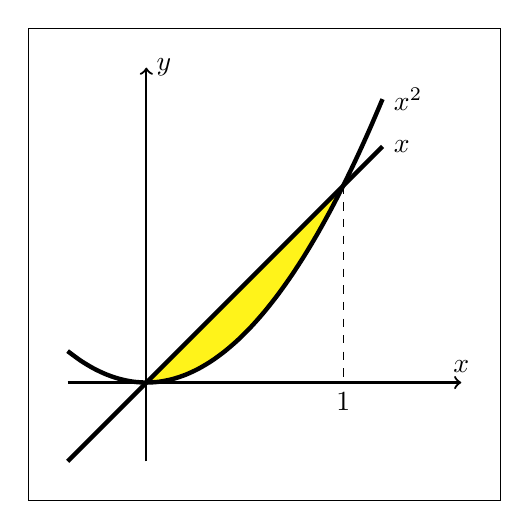
\begin{tikzpicture}
  \draw[fill=white] (-1.5,-1.5) rectangle ++(6,6);

  % shade region
  \draw[fill=yellow!90] plot[smooth, samples=100, domain=0:2.5 ] (\x,0.4*\x*\x) -- (0,0) -- cycle;

  % draw axes
  \draw[thick,->] (-1,0) -- (4,0) node[above] {$x$};
  \draw[thick,->] (0,-1) -- (0,4) node[right] {$y$};

  % draw curves
  \draw[ultra thick,domain=-1:3,smooth,variable=\x,black] plot ({\x},{0.4*\x*\x}) node[right] {$x^2$};
  \draw[ultra thick, domain=-1:3,smooth,variable=\x,black] plot ({\x},{\x}) node[right] {$x$};
        
  \draw[dashed] (2.5,2.5) -- (2.5,0) node[below] {1};
\end{tikzpicture}
\end{document} 
